\documentclass[11pt]{article} % do not change this line
\input{BigDataStyle.txt}      % do not change this line
\usepackage{amsmath,amsfonts,amssymb,amsthm,latexsym,graphicx,array,multicol}

\emergencystretch=5mm
\tolerance=400
\allowdisplaybreaks[4]

\theoremstyle{plain}
\newtheorem{theorem}{Theorem}[section]
\newtheorem{proposition}[theorem]{Proposition}
\newtheorem{corollary}[theorem]{Corollary}
\newtheorem{lemma}[theorem]{Lemma}
\newtheorem{problem}[theorem]{Problem}

\theoremstyle{definition}
\newtheorem*{remark}{Remark}

\title{GOA-KNN: Electronic Annotation of Gene Ontology Terms}
\author{Daniel Syomichev}

\newcommand{\Programme}{Data Science and Analytics}
% Computational Finance students: uncomment the next line
%\twodepartmentstrue

\begin{document}
\maketitle

\declaration;

\begin{abstract}
\end{abstract}

\section{Introduction}

The primary goal of this project is to provide a tool which, given an arbitrary biomedical text, returns a ranked list of Gene Ontology (GO) \cite{ashburner/2000/gene,consortium/2025/gene} terms that characterize the text. The program is intended as a direct substitute to the GOCat project by Gobeill et al. \cite{gobeill/2013/managing}, and functions on the identical premise that GO terms already attributed to a biomedical text can be used to infer the annotations of a new text through the use of the nearest-neighbors algorithm.

\subsection{The Gene Ontology}

The Gene Ontology (GO) \cite{consortium/2025/gene} is a hierarchical vocabulary aimed at categorizing and standardizing biological terminology, particularly with regard to the properties of gene products. The motivation behind the GO "is to produce a dynamic, controlled vocabulary" which is applicable even as the knowledge base changes \cite{ashburner/2000/gene}. Structurally, it is a set of Directed Acyclic Graphs (DAG), with specificity increasing proportionally with distance from the root node; a node represents a term, with relations represented by edges of the graph.

Each of the three roots, referred to officially as "aspects", represent different elements of a gene process: Molecular Function, Cellular Component, and Biological Process. No term appears in more than one aspect, but relations may reference terms contained in different aspects.

\subsection{Biomedical Annotations}

The immense quantity of available biomedical literature creates significant difficulties in efficiently searching and parsing relevant information. This has led to the widespread adoption of tools which are capable of classifying documents and extracting valuable information from them \cite{hunter/2006/biomedical}.  An annotation is an assertion between a gene product and terms within an ontology \cite{hill/2008/gene}, and manual curation of annotations is a time-consuming task. Automatic or electronic annotations are commonly used to provide a "large number of high-quality functional annotations across a broad taxonomic range." \cite{huntley/2014/database} For many species, they are the sole source of annotations available \cite{huntley/2014/database}.

The Gene Ontology Annotation (GOA) project from the European Bioinformatics Institute \cite{huntley/2014/database} aggregates annotations into a singular point of reference, combining both manual annotations from the Gene Ontology Consortium (GOC) and a total of nine electronic annotation pipelines. Most annotations in the dataset contain a literature reference which supports the existence of the annotation \cite{hill/2008/gene}. Informally, the GOA dataset can thus be considered as a mapping from a specific publication to a GO term by exploiting this property of the dataset.

\subsection{GOCat}

Early approaches to electronic annotation of GO terms were thesaurus or dictionary based, utilizing lexical matching of GO term descriptors and synonyms and the input text. This methodology is limited by the representation of a term within text, where it does not often match to the highly precise label within the ontology \cite{gobeill/2013/managing}. The GOCat tool was developed by Gobeill et al. at the University of Geneva \cite{gobeill/2013/managing} in order to address this limitation of dictionary-based approaches. The tool compared an arbitrary input text against a corpus of annotated publication abstracts indexed using the Terrier Platform \cite{ounis/2006/terrier}. Results were scored using the BM25 algorithm \cite{amati/2009/bm}, and the annotated terms of the highest-scoring neighbors were collected and weighed according to similarity. The aggregate scores were then sorted to yield the final ranked prediction. Using the mean reciprocal rank (MRR) as a precision metric and the macro average recall (MAR), the KNN approach consistently outperformed the dictionary-based method.

GOCat is no longer officially available; serving as the primary justification for the development of this project. The quantity of both biomedical text and annotations linking that text to GO terms has substantially increased, and the high availability of pre-train language models provides an alternative indexing method to evaluate. The representation of a document is treated as in independent parameter within the experiment, allowing direct comparisons between indexing methods. In place of the Terrier Platform, this project utilizes a term and inverse document frequency sparse vector representation, and implements a dense representation using embeddings produced by the BiomedBERT model \cite{gu/2021/domainspecific}, trained from scratch on biomedical text. The secondary goal of this project is to evaluate the effectiveness of the sparse representation model over time, and compare it to the embedding representation from a modern language model.

\subsection{Terminology and Notation}

Presented below is a glossary which describe the terminology used throughout this report. In order disambiguate certain concepts, alternate words are utilized to represent different concepts with similar or same naming schemes.

\begin{table}
    \centering
    \begin{tabular}{| m{7.5em} | m{15em} |}
        \hline
        Terminology   & Description                                                   \\
        \hline
        \hline
        term          & Specifically used to reference a GO term.                     \\
        \hline
        token         & Used to reference a term in any other context. (TF-IDF terms) \\
        \hline
        document      & A biomedical text abstract.                                   \\
        \hline
        vectorization & The vector representation of a document.                      \\
        \hline
    \end{tabular}
    \caption{Terminology}
    \label{tab:terminology}
\end{table}
!!TODO!!:
Define conditional statements in sum here...

terms:

tf
tf-idf
idf
bert

ststic embedding
contextual embedding

\section{Research}

This section provides a detailed overview of the concepts used throughout the project. Specific implementation details will be omitted and described in the following section, providing a delineation between theory and application.

\subsection{Term Frequency and Inverse Document Frequency}

In order to compute the scalar distance between two arbitrary text documents, they must be translated into some $p$ dimensional real vector space where the dot product is defined. There are a number of methods to achieve this, but the most applicable to this project is the TF-IDF method. An extension of the bag-of-words method \cite{kim/2019/multicotraining}, it translates each document into a vector with dimensionality equal to the number of tokens in the corpus vocabulary. Each feature is equivalent to the representation of a token within the document, weighed by the representation of the token across the corpus. Adapting the description from Robertson \cite{robertson/2004/understanding}, a token appearing in many documents, such as "protein" across the corpus of article abstracts, is not a good differentiator of documents and the feature attributed to the token within the vector representation should be small.

\subsubsection{Definitions}

A corpus $D$ is a set of documents where each document is represented by a bag of tokens $d = \{t_1, t_2, t_3,...\}$. Defining the frequency of  $t$ within $d$ by $\operatorname{tf}_{t,d} = \sum_{t_i\in d} 1[t_i = t]$ and the frequency of $t$ within $D$ as $\operatorname{df}_{t, D} = \sum_{d\in D} 1[t \in d]$ \cite{manning/2008/scoring}.  The IDF is an extension of the latter definition, and assigns a token to a weight which is inverse proportional to it's frequency within the corpus. First described by Jones in 1972 \cite{jones/1972/statistical}, the definition provided by Manning et al.  \cite{manning/2008/scoring}  has the form:

\begin{equation}
    \operatorname{idf}_{t, D} = \log{\frac{|D|}{\operatorname{df}_{t, D}}}
    \label{eq:idf}
\end{equation}

From these definitions, the score of a token within a document can be calculated as $\operatorname{Score}(t, d, D) = \operatorname{tf}_{t,d} \cdot \operatorname{idf}_{t, D}$, the representation of the token within the document, weighed by the inverse of it's representation within the corpus.

\subsubsection{Score Evaluation}

The vocabulary for a corpus $V_D$ can be defined as the set of unique tokens appearing within the corpus. Let $p = |V_D|$ such that each token in the vocabulary corresponds to an arbitrary dimension in the vector space.  The static embedding \cite{jurafsky/2026/speech}, the vector representation of $d$,  can be computed by first setting a fixed ordering of the vocabulary $V'_D = (v_1, v_2, ..., v_p)$. Then the static embedding is computed by:

\begin{equation}
    x_d = (\operatorname{Score}(v_1,d,D), ... , \operatorname{Score}(v_p,d,D)) \in \mathbb{R}^p
    \label{eq:tfidf_vectorization}
\end{equation}

\subsection{Language Models}

Language models offer an alternative strategy of translating raw text documents to a real vector space through the context of a document as opposed to it's lexicographic properties. The vector representations of documents computed in this manner are called contextual embeddings \cite{jurafsky/2026/speech}. The BERT family of language models, first introduced by Devlin et al. \cite{devlin/2018/bert} in 2018 provide a framework to contextualize the information encoded throughout the entirety of an input sequence, as opposed to auto-regressive models, which only consider the information from earlier in the sequence \cite{jurafsky/2026/speech}.

\subsubsection{Tokenization}

In order to infer contextual embeddings from a BERT model, the input must first be tokenized, a process that is handled by the WordPiece algorithm developed by Wu et al \cite{wu/2016/googles}. Utilizing a fixed subword vocabulary, the input is recursively split on the longest subword which appears in the vocabulary and unknown tokens are replaced by a special token. Each token in the vocabulary has a corresponding identifier which can be used to reference the token in lieu of it's character-based representation \cite{wu/2016/googles}.

The final input representation of a token is the sum of the learned token, segment and positional embeddings. The token embedding encodes the context-free identity of the token \cite{kubek/2025/selfimproving}, the segment embedding delineates the sentence boundary for paired inputs \cite{huang/2021/multiplicative}, and the positional embedding distinguishes the tokens position within the input sequence \cite{huang/2021/multiplicative}. The input representation of a token depends only on it's identity and position, the contextualization is produced by the attention layers of the model.

\subsubsection{Attention}

The BERT model architecture uses bidirectional self-attention, meaning each token attends to the context across the entire sequence. This ensures each token embedding is a reflection of the token's context within the input sequence \cite{devlin/2018/bert} . Define the quantity $H$ representing the hidden size. Let a document be a sequence of tokens $ t_1,t_2, t_3,..., t_n$ with $t \in \mathbb{R}^H$, which form a matrix such that $T \in \mathbb{R}^{n \times H}$.  Let $W^Q$, $W^K$, $W^V$ be learned parameters, such that $Q = TW^{Q}$,  $K = TW^{K}$  and $V = TW^{V}$ \cite{jurafsky/2026/speech}. Each attention head then computes:

\begin{equation}
    \operatorname{Attention}(Q, K, V) = \operatorname{softmax} \left( \frac{ QK^{\top} }{ \sqrt{d_k} } \right) V
    \label{eq:attention}
\end{equation}

The value $d_k$ is the dimensionality of vectors $k \in K$ and $q \in Q$ and is a scaling factor found by Vaswani et al. to prevent the softmax function from being pushed into regions with small gradients \cite{vaswani/2017/attention} .

\subsubsection{Mixed Domain vs. Domain Specific Pretraining}

There exist two distinct methods to pretraining a domain specialized BERT model: mixed domain and domain specific. Mixed domain pretraining essentially initializes the original BERT model, which was pretrained on Wikipedia and BookCorpus \cite{devlin/2018/bert}, and continuing the pretraining process on in-domain text. Domain specific instead trains the model from scratch using only the in-domain text \cite{gu/2021/domainspecific}.  Gu et al. found that domain specific pretraining significantly outperformed mixed domain pretrained model, particularly in domains with an abundance of available literature \cite{gu/2021/domainspecific}.

\subsubsection{The Anisotropic Phenomenon}

First described by Gao et al. \cite{gao/2019/representation}, the problem of anisotropy refers to the uneven distribution of contextual embeddings within a the vector space. Geometrically, the vectors are not distributed uniformly within the vector space, instead occupying a narrow cone \cite{ethayarajh/2019/contextual}. Using direction-based similarity metrics then results in a positive correlation between any two unrelated words \cite{gao/2019/representation}. Ethayarajh also showed that the anisotropy of embeddings grows with each consecutive model layer \cite{ethayarajh/2019/contextual}.

Stollenwerk et al. propose a mitigation strategy they describe as output embedding center (OEC), which involves centering the mean output embedding at the origin \cite{stollenwerk/2026/output}. This is done by subtracting the mean output embedding from each output embedding, effectively normalizing the magnitude around zero. Biś et al. found that output embeddings tend to be isotropic around their center \cite{bis/2021/much}, suggesting the mean centering strategy restores the isotropic property necessary for direction-based comparison.

\subsection{Cosine Distance}

The cosine distance $s$ is defined by:

\begin{equation}
    s = 1 -  \frac{A \cdot B}{\Vert A \Vert \Vert B \Vert}\ \textnormal{where} \  s \in [0, 2]
    \label{eq:cosine_distance}
\end{equation}

In this representation, the distance metric is a method of vector orientation as opposed to magnitude, and is a simple remapping of the cosine similarity. While not a true distance metric, it is a commonly used representation of the semantic similarity of text documents \cite{you/2025/semantics}.  Unlike the Euclidean distance, the cosine distance is invariant to magnitude, neutralizing the influence of the length and absolute frequency of terms in the document.

\subsection{Evaluation Metrics}

In the implementation of GOCat, the prediction was ranked sequence of terms, truncated to a maximum allowed length. By contrast, the true labels were an unordered, arbitrary length set, without any internal ranking scheme. The ontology itself is also hierarchical by construction, implying the possibilty of the classifier predicting a child or parent of the true term. These predictions are not wrong in the binary sense, since there is a relationship between the two terms the classifier may have learned. In order to accurately measure the peculiarities of the task, two sets of metrics are applicable.

Let $D_{test}$ represent the set of test documents, such that $T_d=\{ t_1, ..., t_n \}$ is the set of terms associated with document $d \in D_{test}$, and $\hat{T}_d=(\hat{t}_1, ... , \hat{t}_m )$ be the ranked prediction sequence returned by the classifier.

\subsubsection{Exact Matching}

The first set of metrics treats the label space of terms to be independent of one another, only considering exact matches during evaluation. Used Gobiell et al. to evaluate GOCat, these two metrics represent the model's ability to exactly predict the desired label space, with no consideration for the hierarchical nature of the ontology.

The mean reciprocal rank (MRR) measures the mean position at which the ranked sequence provides a correct prediction across the set of test documents \cite{radev/2002/evaluating}. Formally, define the rank set of a prediction sequence to be $\hat{R}_d = \{  i : \hat{t}_i \in T_d \}$, such that it contains the rank of each correctly predicted term in $\hat{T}_d$. The reciprocal rank and MRR can then be defined by:

\begin{multicols}{2}
    \begin{equation}
        \hat{r}_d =
        \begin{cases}
            0                    & \textnormal{if } |\hat{R}_d| = 0 \\
            (\min\hat{R}_d)^{-1} & \textnormal{otherwise}
        \end{cases}
        \label{eq:rr}
    \end{equation}
    \break
    \begin{equation}
        \operatorname{MRR} = \frac{1}{|D_{test}|} \sum_{d \in D_{test}} \hat{r}_d
        \label{eq:mrr}
    \end{equation}
\end{multicols}

The macro-average recall (MAR) measures the per-term proportion of the case that a term was both associated to a document and predicted to be so. Let $Y_{test} = \bigcup_{d \in D_{test}} T_d$ be the set of all terms associated with documents in the test set. Then for each term, define $F_t = \{d : t \in T_d\}$ and $G_t  = \{ d:t \in \hat{T}_d\}$ to be the sets of documents that contain the term $t$ appearing in the true and predicted sets respectively. Then the MAR can be computed by:

\begin{equation}
    \operatorname{MAR} = \frac{1}{|Y_{test}|} \sum_{d \in D_{test}} \frac{|F_t \cap G_t|}{|F_t|}
    \label{eq:mar}
\end{equation}

Importantly, each term contributes equally to the average, so terms which are disproportionally represented within the test set are not given precedence.

\subsubsection{Hierarchical}

The deficit of the above metrics is the lack of consideration for the relationship between terms. A term which sits one level above the expected term scores just as badly as a term which appears in a separate aspect altogether, which invalidates the ontology's structure entirely. Verspoor et al. demonstrated that the standard multi-label evaluation metrics of precision, recall and F-score report poor performance due to this lack of consideration \cite{verspoor/2006/categorization}, and propose extensions to these metrics which take the strength of the relationship between terms into account. Here ${\uparrow} t$ and ${\uparrow} \hat{t}$ represent the lineage expansions of a true and predicted term respectively. In plain words, these are the sets containing a term and all of it's ancestors.

\begin{multicols}{2}
    \begin{equation}
        \operatorname{HP} = \frac{1}{|\hat{T}_d|} \sum_{\hat{t} \in \hat{T}_d} \max_{t \in T_d} \frac{|{\uparrow} t \cap  {\uparrow} \hat{t}|}{|{\uparrow} \hat{t}|}
        \label{eq:hp}
    \end{equation}
    \break
    \begin{equation}
        \operatorname{HR} = \frac{1}{|T_d|} \sum_{t \in T_d} \max_{\hat{t} \in \hat{T}_d} \frac{|{\uparrow} t \cap  {\uparrow} \hat{t}|}{|{\uparrow} t|}
        \label{eq:hr}
    \end{equation}
\end{multicols}

The hierarchic F-score is the harmonic mean of the two metrics, representing the trade-off between the two.

\begin{equation}
    \operatorname{HF} = 2 \frac{\operatorname{HP} \cdot \operatorname{HR}}{\operatorname{HP} + \operatorname{HR}}
    \break
    \label{eq:hf}
\end{equation}

For hierarchical precision, this definition makes the several key distinctions which make it suitable for evaluating hierarchical predictions. First, there is an increased penalty for predicting an incorrect general term, as opposed to a specific one. The penalty is also proportional with the distance between a predicted term and nearest expected ancestor \cite{verspoor/2006/categorization}. The use of the maxima within the equations ensures that each term is only compared against it's closest match, as opposed to an average over all possible terms \cite{verspoor/2006/categorization}.

Verspoor et al. describe the characteristics of the metrics by comparing situations where there is a single prediction and single truth. If the prediction is a descendant of the expected term, then $HR=1$ and $HP<1$. In the opposite situation, where the prediction is an ancestor of the expected term, $HR < 1$ while $HP=1$. Thus a classifier which scores highly on $HR$ and poorly on $HP$ is generally predicting terms which are more specific than expected and vice versa \cite{verspoor/2006/categorization}.

\subsubsection{Comparability}

MRR, HP, HR and HF are defined per document, and then averaged over the whole test set, while MAR is defined per-term and averaged over all terms in the test set. Therefore, the former metrics are independent of the test set but the MAR is defined only over the entire test set and cannot be depicted as the mean of per document scores.. As a result, it is inaccurate to compare MAR and HR, despite both representing a form of recall. Gobiell et al. treated MRR as a precision metric in their tests \cite{gobeill/2013/managing}, but due to it's construction around rank sensitivity, it cannot be compared to the HP metric. Lastly, the hierarchical metrics are not comparable to their standard counterparts. Verspoor et al. note that "HP and HR will always be higher than the corresponding P and R values for a given test set" and are "not comparable metrics." \cite{verspoor/2006/categorization},

\section{Implementation}

This section contains details specific to the implementation of the program, detailing design decisions which were made based on observed patterns rather than rooted in a research basis.

\subsection{Embedding}

The program provides two independent classes which embed an input document, the \verb|TfidfVectorizer| from SKLearn \cite{pedregosa/2011/scikit-learn}, and a custom \verb|BertEmbeddingsVectorizer| which implements the SKLearn transformer interface in order to fully integrate into an SKLearn workflow \cite{buitinck/2013/api}.

\subsubsection{Text Preprocessing}

Used only in TF-IDF vectorization, the tokenization process standardizes the vocabulary of the corpus, and prevents commonly used words that carry minimal meaning from dominating the frequency aggregates. The general process follows that of Gobeill et al. \cite{gobeill/2013/managing}, though slightly more complex than described in that work.

The first stage of this process is the removal of apostrophes, punctuation unique in that it appears within a word and cannot be treated as a separator. This is important because the tokenization stage collects words which contain at least a single alphabetical and any number of numerical characters, split by whitespace or punctuation.

Alphabetical tokens are reduced to root form using the Porter stemming algorithm \cite{porter/1980/algorithm}. By combining the variants of a token into a single feature, the dimensionality of the vector space is minimized. Alphanumerical tokens are deliberately not stemmed as the algorithm incorrectly strips characters from certain tokens, which then partially lose contextual meaning. To provide a concrete example using a term from the GO:

\[\textnormal{"Rpd3S complex"} \rightarrow \{\textnormal{rpd3s}, \textnormal{complex}\} \rightarrow  \{\textnormal{rpd3}, \textnormal{complex}\}\]

Once the tokens have been stemmed, they are filtered against a stop-word list, which contains some of the most common English language words. Both the Porter stemming implementation and the stop-word list are provided by the NLTK library \cite{loper/2009/natural}. The preprocessing pipeline is utilized symmetrically across vectorization points within the program, meaning training and testing inputs are tokenized identically. Due to the large number of repeated stemming inputs, the function is memoized using the \verb|@functools.cache| decorator.

\subsubsection{Term and Inverse Document Frequency}

The implantation of the SKLearn's \verb|TfidfVectorizer| uses a two step process in order to produce sparse static embeddings. The first step involves computing the vocabulary and the IDF vector of the corpus. The IDF calculation differs from that of Equation \eqref{eq:idf}  by accounting for zero divisions:

\begin{equation}
    \operatorname{idf_{t, D}} = \log {\frac{|D| + 1}{\operatorname{df}_{t, D} + 1}} + 1
    \label{eq:sklearn_idf}
\end{equation}

Once the vocabulary and IDF vector have been computed, they can be stored and later re-initialized into a \verb|TfidfVectorizer| object in order avoid recomputing the values. Recomputation is necessary on any change in the corpus, such as adding a new document. With the vocabulary and IDF vector initialized, raw text can now be transformed into a sparse static embedding using the procedure detailed above.

\subsubsection{BiomedBERT}

The model chosen as the default for this project was BiomedBERT \cite{gu/2021/domainspecific}, a BERT \cite{devlin/2018/bert} variant trained from scratch on abstracts from PubMed and full text articles from PubMedCentral \cite{sayers/2024/database}. This can be changed at any time by supplying the constructor with a valid HuggingFace model name, or the path to the model on disk.

Utilizing the Transformers library from Wolf et al. \cite{wolf/2020/transformers}, the model is automatically initialized with the correct configuration. Each document in the batch is transformed into a sequence of tokens, and truncated to the maximum sequence length, 512 tokens  \cite{sun/2019/finetune},  tolerated by the model. Each sequence shorter than the maximum sequence length across the batch is padded, ensuring the batch of sequences is rectangular.

The values of the last hidden state are the desired per-token contextual embeddings, which are aggregated by the mean-pooling strategy described by Reimers et al \cite{reimers/2019/sentence-bert}. As documents within a batch may be padded, the mean is computed over only the tokens marked as relevant by the attention mask produced by the tokenizer \cite{wolf/2020/transformers}.

Given a batch $D$ of documents $d = \{t_1, t_2, t_3, ...\}$, each a sequence of tokens with attention mask $a = (a_1, a_2, a_3, ...)$ such that $a_i \in \{0, 1\}$, the model returns a sequence of contextual embeddings $e_1, e_2, e_3,...$ where $e_i \in \mathbb{R}^{768}$ \cite{gu/2021/domainspecific, devlin/2018/bert}. The resulting document embedding vector is the mean pool of each token vector, with respect to the attention mask:

\begin{equation}
    e = \frac{\sum_{i} e_ia_i}{\sum_{i} a_i}
    \label{eq:mean_pool_attention_mask}
\end{equation}

This results in a dense vector such that $e \in \mathbb{R}^{768}$, which is representative of the input document, and independent of the corpus.

\subsection{Classification}

The main prediction mechanism of the program utilizes a brute-force KNN algorithm provided by SKLearn's NearestNeighbors estimator to calculate the cosine distance from the vectorized test document to each document vector in the corpus, followed by a weighed voting process to rank each of the predicted terms.

\subsubsection{Neighbor Voting}
The KNN algorithm computes an ordered sequence of document/distance pairs $\{(d_k, s_k) : k \in [1, K]\}$ for a test document $d_{test}$ such that $s_k \in [0,2]$. This sequence represents the prediction and can be unpacked into the sequences of documents $D_K$ and distances $S_K$. Let the sequence of scores be the transformation of distances defined by:

\begin{equation}
    S'_K = \{ (1-s_k)^{\rho} : \rho \in \{1,3,5,...\} \}
    \label{eq:amplified_similarity}
\end{equation}

This process reverts the distance back to a similarity, and then takes it to an exponent $\rho$; a method proposed by Breese et al. \cite{bresse/1998/emprirical}. This technique emphasizes closer matches while punishing further matches. In order to prevent sign degeneration, $\rho$ must be an odd integer.

With $T_d$ as the set of GO terms annotated to a document $d$, the score for a term $t$ is calculated by:

\begin{equation}
    \operatorname{score}(t) = \sum_{(d_k, s'_k)}s'_k\ [t \in T_{d_k}]
    \label{eq:prediction_score}
\end{equation}

Each term annotated to a document in the prediction set is scored and then the list of terms is sorted by the aggregate score, representing the final prediction sequence $T_{d_{test}}$.

\section{Methodology}

This section describes the acquisition and cleaning of the data used to build and validate the program, as well as the protocol used to provide a persistent corpus index.

\subsection{Data Sources}

This project relies upon three sources of data, each of which accommodates a distinct function. The GO is obtained through the basic release from the GOC \cite{consortium/2025/gene},  which is filtered to maintain the acyclic property. The basic variant also contains no cross-aspect relations, allowing safe propagation up the hierarchy. Annotations are obtained from the latest GOA \cite{huntley/2014/database, barrell/2009/database} UniProt archive release which includes the complete cross-species annotation set. The annotation archive provides reference identifiers used to support the existence of an annotation, which are used to acquire article abstracts available through PubMed \cite{sayers/2024/database}.

\subsection{Database Construction}

All information storage is handled by an SQLite database stored locally on disk. The data populated in four distinct stages, three of which are independent of one another. The terms| and \verb|relations| tables are assembled from the ontology basic release and the \verb|annotations| table from the annotation archive. Once the \verb|annotations| table is constructed, the distinct PubMed identifiers (PMID) within it are used to query the NCBI E-Utilities \cite{sayers/2024/database} service for abstracts, populating the  \verb|citations| table.

\subsubsection{Ontology}

The GO release is in essence a flattened representation of a graph, structured as a list of nodes representing terms and their metadata, alongside a list of edges which represent the relations between nodes. The \verb|terms| table is a mapping from GO identifier (GOID) to the human-readable term name; the prefix to each GOID consisting of "GO:" is removed and each GOID is stored as an integer. The \verb|relations| table stores the edges of the graph, allowing for a full reconstruction of the graph from the data stored in the database.

\subsubsection{Annotations}

The annotation archive is of a tab-delimited format and read line-by-line, extracting three relevant fields from each: the GOID associated with the annotation, the database reference and the date of the annotation. Database references which do not contain a PMID are discarded, removing annotations which are supported by sources other than literature. The remaining rows assert a connection between a publication and the GO term, alongside the date of when that connection was established. Due to the nature of the GOA archive, the same pair of GO term and publication may appear, requiring a conflict resolution strategy. Any conflicting pair of GOID/PMID combinations are overwritten, with the earliest annotation date taking priority.

\subsubsection{Citations}

The distinct PMIDs appearing in the \verb|annotations| table are resolved to an article's abstract through the \verb|e-fetch| endpoint of the E-utilities service. Requests are batched and limited to the rate published in the documentation; 10 requests per second with a provided API key, and three otherwise. Batches will retry up to three times before raising an exception,  under the assumption that something went wrong in transit as opposed to a configuration error.  Due to the long running nature of this process, batches will only contain PMIDs which are not already populated in the \verb|citations| table, allowing a safe restart if the process fails.

The batch response is contained in an XML document, which is used to extract the raw abstract text and map it to it's associated PMID. In the case that the abstract has additional formatting or is structured in multiple elements, the text is concatenated to construct a single uniform document, while empty abstracts are ignored.

\subsubsection{Relevant Metadata}
\begin{table}
    \centering
    \begin{tabular}{|m{10em}|m{5em}|}
        \hline
        Attribute         & Quantity \\
        \hline
        \hline
        Terms             & 48,329   \\
        \hline
        Relations         & 71,895   \\
        \hline
        Annotation Pairs  & 554,707  \\
        \hline
        Annotation PMIDs  & 204,622  \\
        \hline
        Annotation GOIDs  & 28,185   \\
        \hline
        Final Corpus Size & 202,638  \\
        \hline
    \end{tabular}
    \caption{Metadata related to quantities of data used during experimentation. }
    \label{tab:metadata}
\end{table}

In addition to Table \ref{tab:metadata}, article abstracts in the corpus span the publication date range of 1959 to 2026, while annotations span the range 1999 to 2026. Out of the 202,638 documents in the corpus, there are three duplicates; each contains the text "[Figure: see text]." and hold valid associations to annotations.

Several properties of the data should also be noted. First, of 48,239 GO terms, only 28,185 are referenced by annotations. Due to the nature of the KNN algorithm, only 58\% of the potential label space is ever visible, meaning over 40\% of GO terms will never be predicted regardless of how well they match the input document. Second, the label space is incredibly imbalanced as seen in Figure \ref{fig:annotation_terms}. Only a small handful of terms are associated with a large majority of annotations, and thus can be expected to be predicted much more frequently.

\begin{figure}
    \centering
    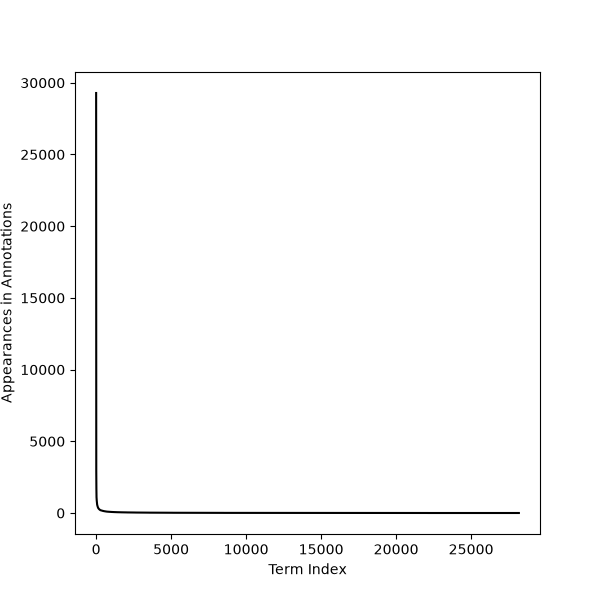
\includegraphics[width=0.5\linewidth]{annotation_term_count.png}
    \caption{Term Index vs. Appearances}
    \label{fig:annotation_terms}
\end{figure}

\subsection{Indexing }

In order to prevent re-indexing each time a query is executed, there exist secondary tables within the database responsible for persistence of an index. Each vectorization method maintains it's own index, and each is treated as a distinct branch in the programs execution path.

The \verb|TfidfVectorizer| is persisted as two separate tables: \verb|vocabulary| and \verb|vectorizations|. The \verb|vocabulary| table stores a token's position within the ordered vocabulary and its IDF value. The \verb|vectorizations| table stores the sparse matrix in COO format keyed on the PMID of the associated document. The sparse matrix is reconstructed and translated into CSR format, the standard used throughout SKLearn, on load. Importantly, the sparse matrix is never materialized, minimizing memory and transfer overhead.

Contextual embeddings emitted by \verb|BertEmbeddingsTokenizer| are stored as a serialized array. Each embedding, a vector in $\mathbb{R}^{768}$, is serialized using the Pickle utility and stored as byte blob. As such, no reconstruction of the vector is necessary upon re-initialization, simply de-serialization. Importantly, due to the anisotropic property of BERT embeddings, the embedding vectors are mean centered before any classification in accordance with the strategy described by Stollenwerk et al. \cite{stollenwerk/2026/output} using SKLearn's \verb|StandardScaler| without scaling to unit variance.

\subsection{Hierarchical Evaluation}

In addition to implementing the two evaluation metrics used by Gobiell et al. when testing GOCat \cite{gobeill/2013/managing}, the classifier is also evaluated using the hierarchical metrics described by Verspoor et al. \cite{verspoor/2006/categorization} by utilizing the relations within the GO. Each of the true and predicted terms are expanded to their full lineage by traversing the 'is a' and 'part of' relations. These relations imply a direct relationship between a child and parent term, as described by the GOC \cite{consortium/2025/gene}  (!!TODO!!: add propper reference to this, it's on the GO website). The process is memoized in-memory using the \verb|@functools.cache| decorator to avoid repeating traversals along the graph. Using these expansions, the HP, HR, and HF scores are calculated according to the formulations previously described.

\section{Experiment}

Three experiments were conducted, and this section describes the results of these experiments, alongside an interpretation of these results based on the conducted research. Each type of metric described in the Research section is reported separately, as it has already been established that they cannot be compared against each other.

\subsection{Hyperparameter Tuning}

There are a total of three hyperparameters which hold sway over the classifier: the number of neighbors $k$, the amplification exponent $\rho$ and the prediction truncation limit $l$. Using the SKLearn \verb|GridSearchCV|, an exhaustive search is performed over the values of $k \in \{ 25, 50, 100, 200 \}$, $\rho=\{1,3,5\}$ and $l=\{5,10,20\}$ across all 36 combinations. Each combination is evaluated over 10 randomly shuffled folds of the full 202,638 document corpus. A fixed random seed is provided in order to ensure identical shuffling for both vectorization methods.

In order to reduce computation time, the \verb|OntologyClassifier| memoizes repeated calls of it's \verb|predict| method to disk. This is achieved by providing the classifier with the maximum value of $k$ across the search $k_{max}$, such that any call to the \verb|predict| internally computes the $k_{max}$ nearest neighbors for a given train and test set. This result is then truncated to the true value of $k$ before any scoring occurs, preserving the validity of the resulting prediction sequence. The memoization is accomplished through JobLib's \verb|Memory| interface, which hashes based on the input parameters of a function. This significantly reduced the running time of the exhaustive search, since the nearest neighbor calculation is performed brute-force, and the number of times this calculation needed to be carried out was reduced from 360 to 10.

The test suite also implements a mock \verb|BertEmbeddingsVectorizer|, which is a wrapper of a simple dictionary based retrieval of a documents embedding by the documents content. The embeddings are precomputed once, and retrieved from the database upon initialization of the script. This prevents the search from re-computing each test documents embedding, and is a valid substitution because an embedding is independent of the overall corpus. In contrast, the \verb|TfidfVectorizer| is refitted for each fold in order to prevent leakage. Once again utilizing JobLib's \verb|Memory| interface, the resulting index and test document vectors are stored on disk, and simply retrieved for each fold as opposed to recomputing them.

\begin{table}
    \centering
    \begin{tabular}{| m{4em} | m{2em} | m{2em} | m{3em} | m{3em} | m{3em} | m{3em} | m{3em} |}
        \hline
        Method & $k$ & $\rho$ & MRR            & MAR            & HP             & HR             & HF             \\
        \hline
        \hline
        TF-IDF & 100 & 3      & \textbf{0.448} & \textbf{0.386} & 0.284          & 0.829          & 0.397          \\
        \hline
        BERT   & 25  & 5      & \textbf{0.419} & \textbf{0.269} & 0.311          & 0.806          & 0.422          \\
        \hline
        \hline
        TF-IDF & 200 & 1      & 0.442          & 0.357          & \textbf{0.299} & \textbf{0.840} & \textbf{0.413} \\
        \hline
        BERT   & 100 & 5      & 0.417          & 0.257          & \textbf{0.326} & \textbf{0.813} & \textbf{0.437} \\
        \hline
    \end{tabular}
    \caption{Optimal hyperparameters for both vectorization methods over the MAR and HF metrics with fixed $l=20$.}
    \label{tab:both_optimal_sel}
\end{table}

As evidenced by table \ref{tab:both_optimal_sel}, the vectorization methods each achieve better results across differing metrics. TF-IDF vectorization scored significantly better with the MAR metric, with a difference of about 0.117, and also outperforms the BERT method by 0.029 on the MRR metric. The interpretation becomes less clear with the hierarchical metrics, as the TF-IDF method outscores the BERT method in HR by 0.07, but is outscored by 0.027 on HP and 0.024 on HF. It is important to note that these patterns hold for the suboptimal hyperparameter values depicted by the non-bold columns of table \ref{tab:both_optimal_sel}.

\begin{figure}
    \centering
    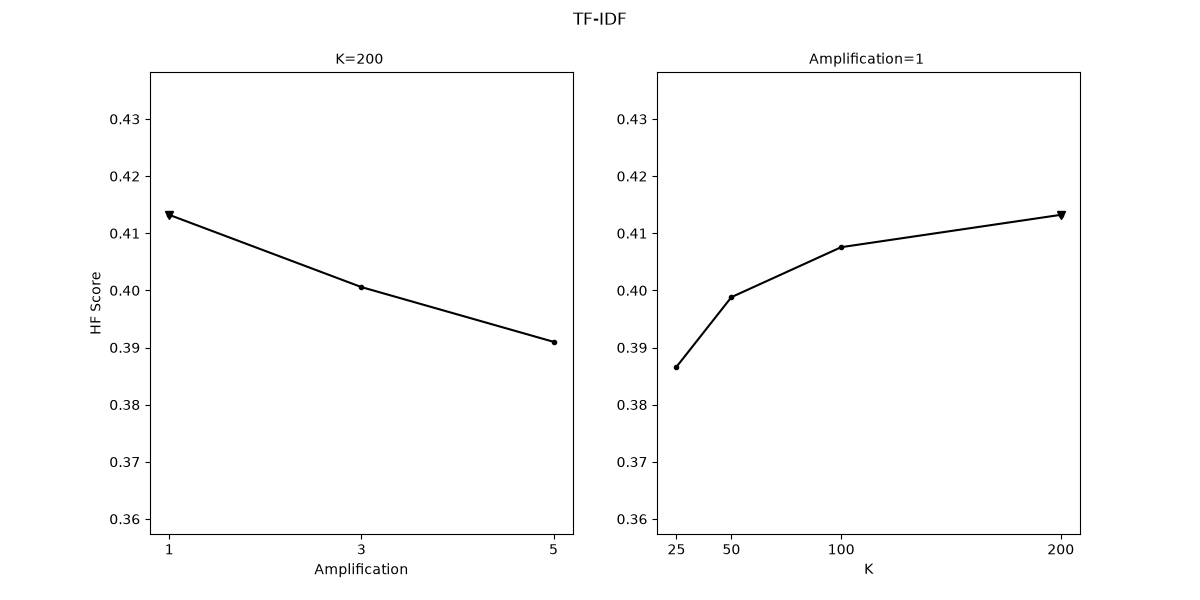
\includegraphics[width=1\linewidth]{hyperparameters_tfidf.png}
    \caption{Hyperparameter trend for TF-IDF vectorization with non-depicted hyperparameters fixed. ($l=20$)}
    \label{fig:tfidf_hyp_trend}
\end{figure}

Trends for the $k$ and $\rho$ hyperparameters are shown by figures \ref{fig:tfidf_hyp_trend} and \ref{fig:bert_hyp_trend}. The non-varied parameter is fixed at it's optimal value maximizing HF. In order to effectively depict the change, the dependent axis has been windowed to the operating range of the score, and the optimal hyperparameter value is plotted with a triangle rather than a dot. The increasing value of $k$ improves the TF-IDF vectorizer with diminishing returns as $k \rightarrow 200$, and differs from the behavior of the BERT vectorizer, which peaks at $k=100$. This suggests that the KNN algorithm is more sensitive for the TF-IDF vectorization, returning more valid neighbors in the tail of the result, while the BERT vectorization returns more unrelated noise.
\begin{figure}
    \centering
    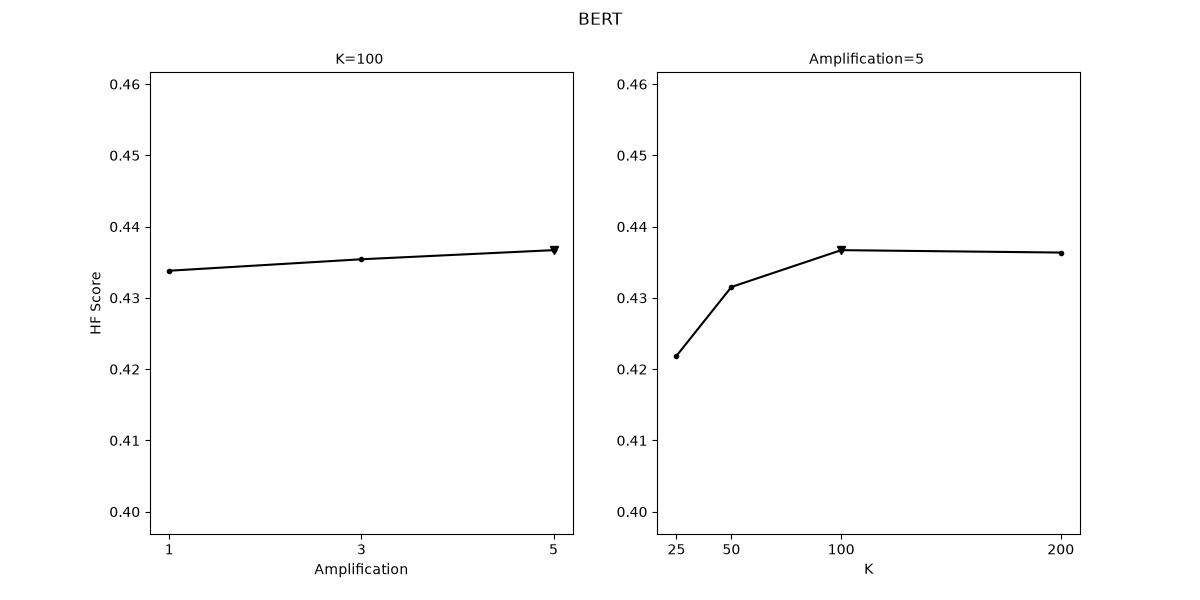
\includegraphics[width=1\linewidth]{hyperparameters_bert.png}
    \caption{Hyperparameter trend for BERT vectorization with non-depicted hyperparameters fixed. ($l=20$)}
    \label{fig:bert_hyp_trend}
\end{figure}

Amplification also behaves differently between the two, such that the TF-IDF scores substantially worse with higher amplification, while BERT prefers $\rho=5$, but only marginally so. This is due to the structural differences between the vectorization methods. Table \ref{tab:mean_distance_at} depicts the mean difference between the nearest neighbor, as well as the mean distance for the 25th neighbor, demonstrating the distribution of neighbors within the space.

\begin{table}
    \centering
    \begin{tabular}{| m{4em} | m{3em} | m{3em} |}
        \hline
        Method & $k=1$  & $k=25$ \\
        \hline
        \hline
        TF-IDF & 0.4536 & 0.7304 \\
        \hline
        BERT   & 0.0036 & 0.0048 \\
        \hline
    \end{tabular}
    \caption{Average distance to nearest neighbor at $k=1$ and $k=25$ across both vectorization methods.}
    \label{tab:mean_distance_at}
\end{table}

This result demonstrates the difference between the two methods. Even accounting for the mean-centering performed on the BERT embeddings, the relative distance between the upper end of the nearest neighbors result shows a very small absolute difference between the distances. When considering to the possible range of cosine distance, the TF-IDF scores differ by about 13\%, while the BERT embeddings differ by only 0.6\%. Because scores are not normalized to a static range, as would be the case if using the min-max normalization scheme, the absolute contribution of a neighbor at $k=1$ and $k=25$ is nearly indistinguishable, which is the reason higher amplification improves the result using BERT vectorization. By accentuating more extreme neighbor similarities, and squeezing near-orthogonal neighbors towards zero, the scoring method is able to distinguish the contributions of closer neighbors. This technique is not effective using the TF-IDF method because the scores are much more uniformly distributed, and amplification instead over-compensates the contributions of closer neighbors. It should also be noted that due to the mean centering strategy, embedding distances can be negative, and contribute negatively to the overall score of the term in the final ranking.

To connect the results in \ref{tab:both_optimal_sel} to the characteristics of the hierarchy metrics described by Verspoor et al. \cite{verspoor/2006/categorization}, it can be inferred that the TF-IDF based classification tends to predict descendants of the expected terms, while the BERT based classification more frequently predicts ancestors.

\subsection{Head to Head}

The comparison's provided by table \ref{tab:both_optimal_sel} are only a selection over the maximal scores of MAR and HF, which are not representative of the exhaustive search as a whole. In order to demonstrate the preference of metric type displayed by each model, a binary representation is provided. Figures \ref{fig:method_h2h_mar} and \ref{fig:method_h2h_hf} represent the parameter selection at each of  $l \in {5, 10, 20}$, for both the MAR and HF metric.

\begin{figure}
    \centering
    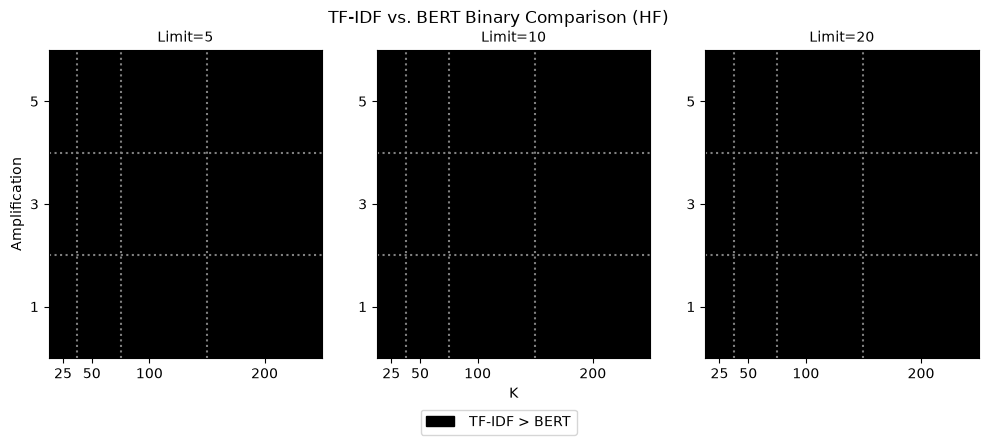
\includegraphics[width=0.75\linewidth]{tfidf_versus_bert_mar.png}
    \caption{Head to head comparison of TF-IDF vs. BERT over MAR metric.}
    \label{fig:method_h2h_mar}
\end{figure}

As evidenced by figure \ref{fig:method_h2h_mar}, the TF-IDF vectorizer presents the better MAR across all 36 combinations, with scores averaged over each of the 10 folds. This indicates that the TF-IDF vectorizer was able to more accurately determine the exact terms annotated to each document in the fold's testing set. This is a per-term score, indicating that uncommon terms were better represented in predictions using the TF-IDF transformation method.

\begin{figure}
    \centering
    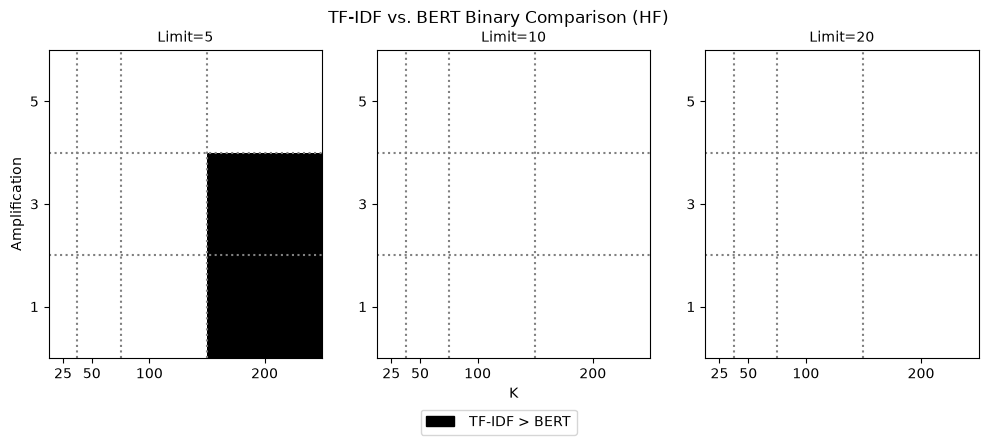
\includegraphics[width=0.75\linewidth]{tfidf_versus_bert_hf.png}
    \caption{Head to head comparison of TF-IDF vs. BERT over HF metric.}
    \label{fig:method_h2h_hf}
\end{figure}

Conversely, the BERT vectorizer scored better over the HF metric across 34 out of 36 combinations. The only outliers were at  $l=5$ and $k=200$, and are truly outliers since at a truncation limit of five, the scoring algorithm cannot effectively filter noise from the aggregation result.

\subsection{Temporal Evolution}

Mirroring the experiment conducted by Gobiell et al. in nature but not in construction, the pseudo-temporal analysis provides a measurement of the classifiers effectiveness as the quantity of available data grows. This is not a true comparison to the results provided by Gobiell et al. \cite{gobeill/2013/managing}, since historic releases of the GO and annotations archive were not utilized. Unlike a true cross validation, the annotations are grouped by their earliest recorded year within the archive, and train/test splits are generated iteratively.

\begin{figure}
    \centering
    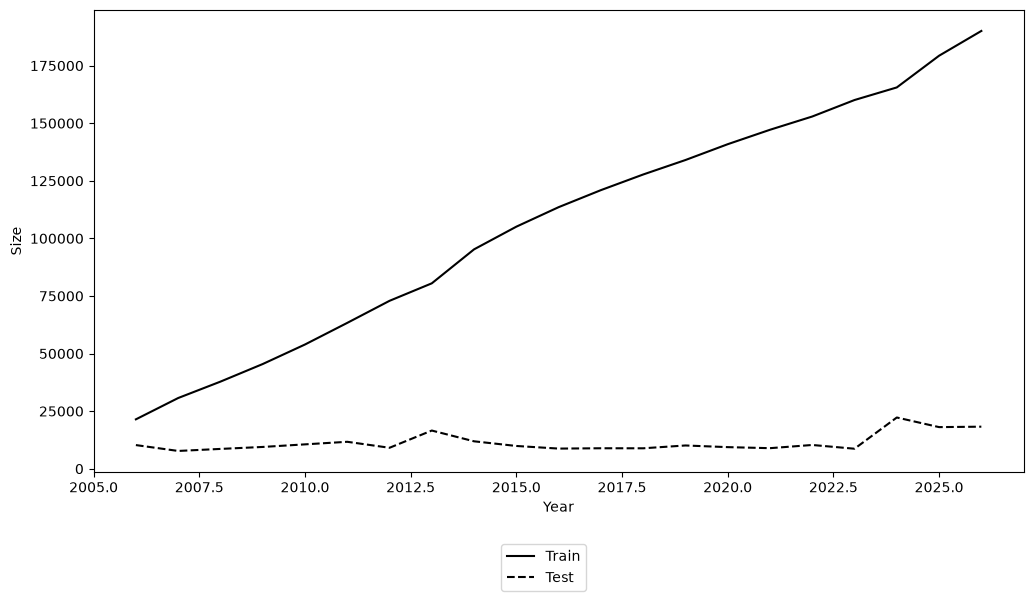
\includegraphics[width=0.75\linewidth]{historical_train_test_split_size.png}
    \caption{Train/Test split sizes per-year for the temporal evaluation.}
    \label{fig:hist_sizes}
\end{figure}

For each year starting in 1999, a nested mapping is constructed per-year per-document such that it is first keyed on the year of annotation, and then the documents PMID. Importantly, this mapping makes distinct the year the annotation was made, rather than aggregating each document's annotations.  If a document was annotated with year term $t_a$  in year $y_a$, and term $t_b$ in year $y_b > y_a$, then the mapping for the document in year $y_b$ will not contain term $t_a$. The testing set only contains the documents with annotations made in that year, while the training set is the union of all previous years. The size comparison of each year is provided in table \ref{fig:hist_sizes}.

Because a document can be annotated to multiple terms over multiple years, the testing set includes the document and all of the terms which were annotated to it in previous years alongside the current year. This potentially introduces leakage of the testing set, since a partially complete set of terms for a document could be present in the training set. To mitigate this, exact matches are excluded entirely from the scoring process, and have no bearing on the final metric scores, which effectively asks the classifier to predict all terms for a document without knowledge of it's annotations from previous years. The test is completed over both the exact and hierarchical metrics in order to showcase the behavioral differences between the two metrics. Each classifier uses it's optimal parameter configurations with a fixed $l=20$.

\begin{figure}
    \centering
    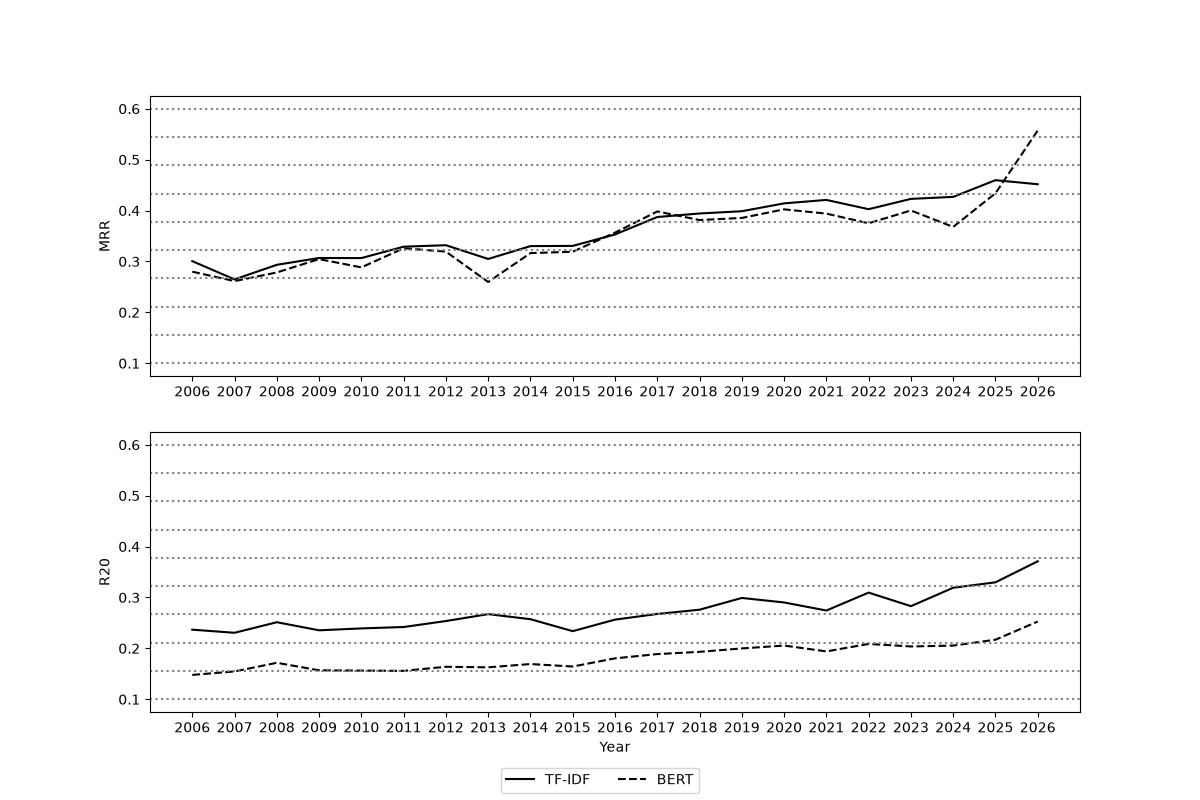
\includegraphics[width=0.75\linewidth]{historical_exact.png}
    \caption{Psuedo-historical comparison utilizing MRR and MAR20, testing on year $i$ and training on years $j<i$.}
    \label{fig:historical_exact}
\end{figure}

The exact metrics generally improve as the number of available annotations grows, with MRR 0.30 in 2006 to 0.452 in 2026 for the TF-IDF method. The BERT method also follows a similar trajectory, rising from 0.280 in 2006 to 0.55 in 2026. This supports the claim that as the quantity of comparison points increases, the ability of the classifier to predict exactly also increases.

\begin{figure}
    \centering
    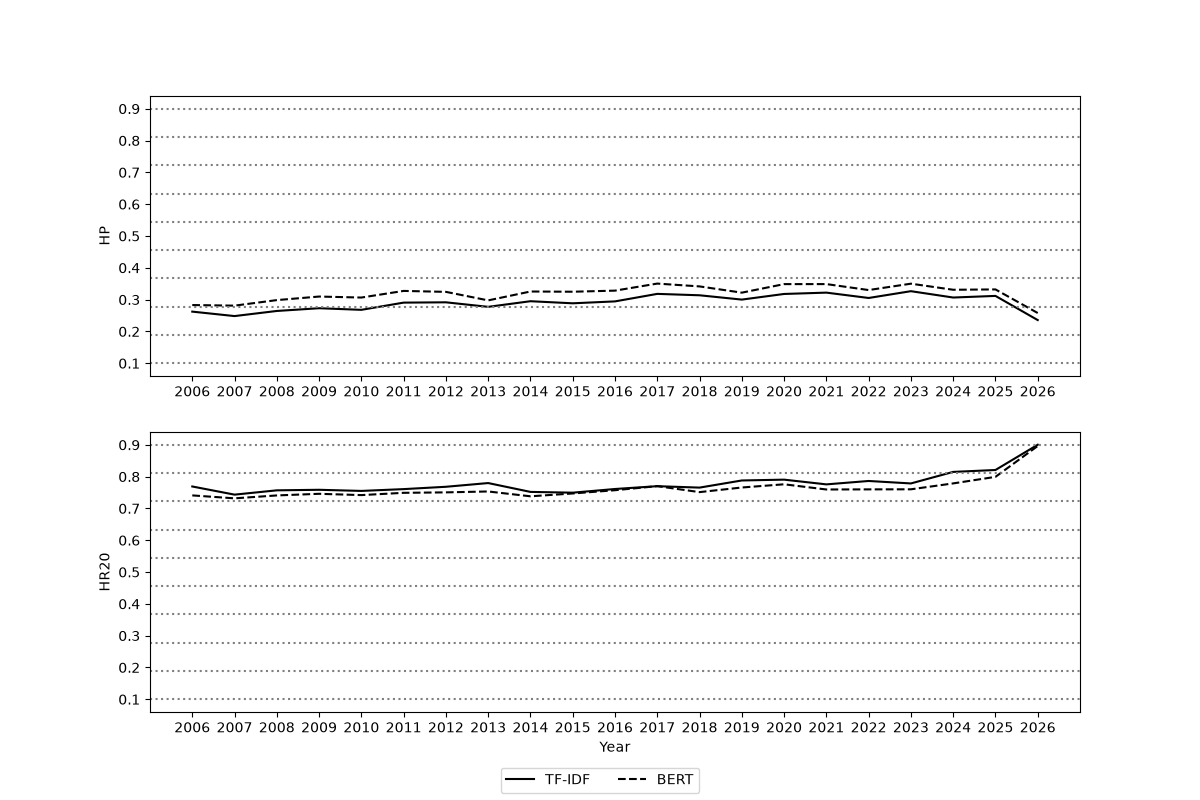
\includegraphics[width=0.75\linewidth]{historical_hierarchical.png}
    \caption{Psuedo-historical comparison utilizing HP and HR20, testing on year $i$ and training on years $j<i$.}
    \label{fig:historical_hier}
\end{figure}

On the other hand, the hierarchical metrics don't seem to be affected by the quantity of annotations available to the classifier. For the TF-IDF method, HF grew from 0.262 in 2006 to 0.312 in 2025, then experiencing a dip in to 0.236 in 2026. The BERT method fares similarly, albeit with higher baseline scores; its HF grew from 0.385 in 2006 to 0.436 in 2025, and also exhibited a drop in 2026 to 0.367. While an elementary application of the characteristics described by Verspool et al. \cite{verspoor/2006/categorization}, the trajectories of hierarchical measures seem to imply that both methods are typically overly specific, predicting descendants of the expected term. The relatively minimal slope of both trends suggests that the classifier was able to correctly predict the lineage of a term, which is reflected positively in the hierarchical metrics, even with minimal comparison points.

\section{Evaluation}

\subsection{Tokenization Complexity}

The tokenization process is a large factor in the success or failure of TF-IDF vectorization. Because the primary indicator of the document is the IDF vector and it's associated vocabulary, the tokens chosen to be a part of the vocabulary play a large role in ensuring the vectorization is an accurate representation of the document throughout the corpus. Leaving too many common tokens results in document vectors which are indistiguishable from one another, while stripping too many away results in a document vector which is so specific to the particular document, it cannot be grouped amonst the other documents in the corpus. This is in essence a partitioning optimization, where the optimal ratio of general to specific must be found in order for the vectorization to be successful.

The current implementation of tokenization stuggles to capture semantic relationships such as synonyms.
The GO explicitly provides a list of synonyms for most terms, which can be understood to imply the commonality of synonymous terminology in biomedicine. In fact, managing the sprawl of synonymous language in biomedical literature is the GO's primary stated purpose. Within the current tokenization process, synonyms are treated independently, and cannot be accurately reflected in the vectorization process as a result. One paper may reference "saposin", while another "sphingolipid activator protein activity" which are synoymous according to the GO, but the tokenizer and by proxy TF-IDF vectorization are incapble of depticting this relationship.

There are also an abundance of other issues pertaining to the tokenization step which are not rooted in the theoretical aspects of the process, but are specifically due to a rather primitive implementation. One prominant example of this is the poor handling of non-contextual strings such as dates, identifiers or postfixes

Given the ontology explicitly provides a list of synonyms, for most terms,

TF-IDF vectorization is largely dependent on the tokenization process which precedes it,

The primary determining factor of TF-IDF vector comparison is the presence of token which are uncommon or "markers" across the corpus. Even under normalization through cosine distance comparison, tokens with higher IDF values will contribute more to the direction of a document vector than common tokens such as "protein" or "cell". This is a valuable property of the vectorization, and ensures that documents containing the similar distributions of marker tokens are grouped together.

\begin{itemize}
    \item tokenization failures for tf-idf, why a more complicated tokenizing process could help but also be more expensive and ultimately subjective.
    \item discuss the failure of using a standard bert model rather than using a sentence-bert variant. Alleviates the Anisotropic problem significantly, while also allowing for per-sentence tokenization which should also capture more context.
    \item discuss cost of using one tokenization method over the other, since tfidf is lower upfront but longer sustained, needing to recompute vocab, idf and vectorizations for each corpus change. bert should realistically be fine-tuned before use, which was not in scope for this project as it's extremely high cost.
    \item discuss a potential extension which utilizes a more involved classification algorithm, potentially a model based classifier instead of the algorithmic knn implementation now.
\end{itemize}

\subsection{Vectorization Trade-Offs}

The primary determining factor of TF-IDF vector comparison is the presence of token which are uncommon or "markers" across the corpus. Even under normalization through cosine distance comparison, tokens with higher IDF values will contribute more to the direction of a document vector than common tokens such as "protein" or "cell". This is a valuable property of the vectorization, and ensures that documents containing the similar distributions of marker tokens are grouped together.

Context and language variation are where this method begins to struggle; Many terms in the ontology are multiple words long, such as "mitochondrion inheritance", and the semantic context between the two cannot be accurately represented within the current tokenization process, at least without significantly ballooning the size of the dictionary. Synonyms are also common across biomedical text, and the sparse dictionary method treats each as entirely unrelated.

The process is dependent on the corpus of documents, alongside the tokenization process. This means that any time a document to the corpus, the transformer must be refitted and the corpus re-vectorized. The cost of adding a document to the corpus scales proportionally to the corpus' size. With a relatively simple tokenization process, this is a computationally cheap task. However, even with the simple process outlined in the implementation of the tokenization process, memoization was required to significantly reduce computation time of the Porter stemming. The more nuance added to the tokenization process, such as re-mapping synonyms, the more expensive the process becomes.

A BERT embeddings vectorization addresses many of the drawbacks of the TF-IDF vectorizer, in that the bidirectional self-attention provides contextual awareness between tokens. A model is theoretically capable of determining that two synonymous GO terms such as "saposin" and "sphingolipid activator protein activity" are contextually linked through the distribution learned from the training data.

This process is entirely dependent on the training of the model and is difficult to quantify or tune. As seen in the experimental data, the BiomedBERT model often scored poorly on recall metrics. The cost of fine tuning the model is significant, requiring heavy computational loads and a massive amount of data. The potential effectiveness of the BERT based approach is high, but the cost of reaching that effectiveness is also much higher than that of the TF-IDF approach.

Even once trained, the model requires significant computation to vectorize the entire corpus; anecdotally hours versus the TF-IDF vectorization's minutes. However, adding a document to the corpus is linear, due to the independence of the vectorization from the corpus. Within the specific implementation of the BertEmbeddingsVectorizer, the truncation of long documents means partial encoding and loss of potentially valuable information; this is a time and priority limitation, rather than a downside of the method.

\subsection{BERT vs. Sentence-BERT}

\subsection{}

\subsubsection{}

\section{Personal Assessment}

\section{Conclusion}

\section{Appendix}

\begin{table}
    \centering
    \begin{tabular}{| m{2em} | m{2em} | m{4em} | m{4em} | m{4em} | m{4em} | m{4em} |}
        \hline
        $k$ & $\rho$ & MRR             & MAR             & HP              & HR              & HF              \\
        \hline
        \hline
        200 & 3      & \textbf{0.4509} & 0.3845          & 0.2874          & 0.8326          & 0.4006          \\
        \hline
        100 & 3      & 0.4484          & \textbf{0.3861} & 0.2841          & 0.8285          & 0.3967          \\
        \hline
        200 & 1      & 0.4418          & 0.3569          & \textbf{0.2991} & 0.8398          & 0.4132          \\
        \hline
        200 & 1      & 0.4418          & 0.3569          & 0.2991          & \textbf{0.8398} & \textbf{0.4132} \\
        \hline
        200 & 1      & 0.4418          & 0.3569          & 0.2991          & \textbf{0.8398} & \textbf{0.4132} \\
        \hline
    \end{tabular}
    \caption{Optimal hyperparameter values maximizing each available metric for the TF-IDF vectorization method with fixed $l=20$.}
    \label{tab:tfidf_optimal}
\end{table}

\begin{table}
    \centering
    \begin{tabular}{| m{2em} | m{2em} | m{4em} | m{4em} | m{4em} | m{4em} | m{4em} |}
        \hline
        $k$ & $\rho$ & MRR             & MAR             & HP              & HR              & HF              \\
        \hline
        \hline
        50  & 5      & \textbf{0.4235} & 0.2677          & 0.3200          & 0.8132          & 0.4315          \\
        \hline
        25  & 5      & 0.4190          & \textbf{0.2688} & 0.3109          & 0.8059          & 0.4219          \\
        \hline
        200 & 5      & 0.4044          & 0.2351          & \textbf{0.3270} & 0.8071          & 0.4364          \\
        \hline
        100 & 5      & 0.4173          & 0.2565          & 0.3258          & \textbf{0.8133} & \textbf{0.4367} \\
        \hline
        100 & 5      & 0.4173          & 0.2565          & 0.3258          & \textbf{0.8133} & \textbf{0.4367} \\
        \hline
    \end{tabular}
    \caption{Optimal hyperparameter values maximizing each available metric for the BERT vectorization method with fixed $l=20$.}
    \label{tab:bert_optimal}
\end{table}

\bibliographystyle{plain}
\bibliography{bibliography}
\end{document}
